\section{Spectrecoin Specifications}
\begin{table}[h]
\resizebox{\textwidth}{!}{%
\begin{tabular}{@{}ll@{}}
	\hline
	\textbf{Genesis block} & Block \#1 mined on 20/11/2016 (later transition to PoS only)\\
	\midrule
	\textbf{Distribution} & ICO that raised 16 BTC w/ subsequent distribution in early 2017\\
	\midrule
	\textbf{Ticker} & XSPEC\\
	\midrule
	\textbf{Initial supply} & 20,000,000 XSPEC\\
	\midrule
	\textbf{Network outputs (public)} & XSPEC – public coins\\
	\midrule
	\textbf{Network outputs (private)} & SPECTRE – private coins\\
	\midrule
	\textbf{Consensus (XSPEC)} & Proof-of-Stake v.3 (PoSv3)\\
	\midrule
	\textbf{Consensus (SPECTRE)} & Proof-of-Anonymous-Stake (PoAS)\\
	\midrule
	\textbf{Difficulty retarget} & Every block\\
	\midrule
	\textbf{Target block time} & 96 seconds\\
	\midrule
	\textbf{Block reward (PoSv3)} & 2 XSPEC\\
	\midrule
	\textbf{Block reward (PoAS)} & 3 SPECTRE\\
	\midrule
	\textbf{Coin maturity (confirmations)} & 450 for stake reward / 10 for SPECTRE / 6 for XSPEC\\
	\midrule
	\textbf{Max supply} & No max supply (see illustrations on page 8)\\
	\midrule
	\textbf{Inflation} & Decreasing over time tending to zero\\
	\midrule
	\textbf{Code repository} & https://github.com/spectrecoin/spectre\\
	\midrule
	\textbf{Supported platforms} / OS & MS Windows, OSX, Linux, Raspberry Pi\\
	\midrule
	\textbf{Website} & https://spectreproject.io/\\
	\midrule
	\textbf{Block explorer} & https://chainz.cryptoid.info/xspec/\\
	\hline
\end{tabular}%
}
\end{table}
\noindent
It is important to understand that the total ‘\textit{outstanding}’ amount is the sum
of \linebreak XSPEC + SPECTRE. On the next page we have projected both a minimum and a
maximum inflation rate and total ‘\textit{outstanding}’ amount of XSPEC + SPECTRE over
20 years. The real value of the total ‘\textit{outstanding}’ amount will depend on the
ratio of XSPEC / SPECTRE created by the two different consensus mechanisms
over time. The minimum values represent a scenario where 100\% of the blocks
are created by PoSv3 and the maximum values represent a scenario where 100\%
of the blocks are created by PoAS.
\newpage


\section{Spectrecoin Characteristics}
The Spectrecoin software is encompassing and integrating the following:

\begin{table}[h]
\resizebox{\textwidth}{!}{%
\begin{tabular}{@{}ll@{}}
\hline
\textbf{Bitcoin Core} & Core technology of the Spectrecoin block-chain. \\ 
\midrule
\textbf{Proof-of-Stake.v3 (PoSv3)} & Secure open consensus mechanism for XSPEC public coins. \\ 
\midrule
\textbf{Proof-of-Anonymous-Stake (PoAS)} & Secure  private  consensus  mechanism  for  SPECTRE private coins. \\
\midrule
\textbf{Private transactions} & Using dual-key stealth technology and ring signatures for SPECTRE. \\
\midrule
\textbf{TOR} & to hide your real IP address (\textit{all Spectrecoin nodes run as hidden services}). \\
\midrule
\textbf{OBFS4} & To hide the fact that you are using TOR to avoid censorship. \\
\hline
\end{tabular}%
}
\end{table}
\noindent
Given the specific specifications and design, Spectrecoin takes on the characteristics of both a Bitcoin like blockchain and a Monero like blockchain. This combined with a pure PoS strategy makes Spectrecoin unique.

\subsection{Inflation rate over 20 years}
\begin{figure}[h]
	\centering
	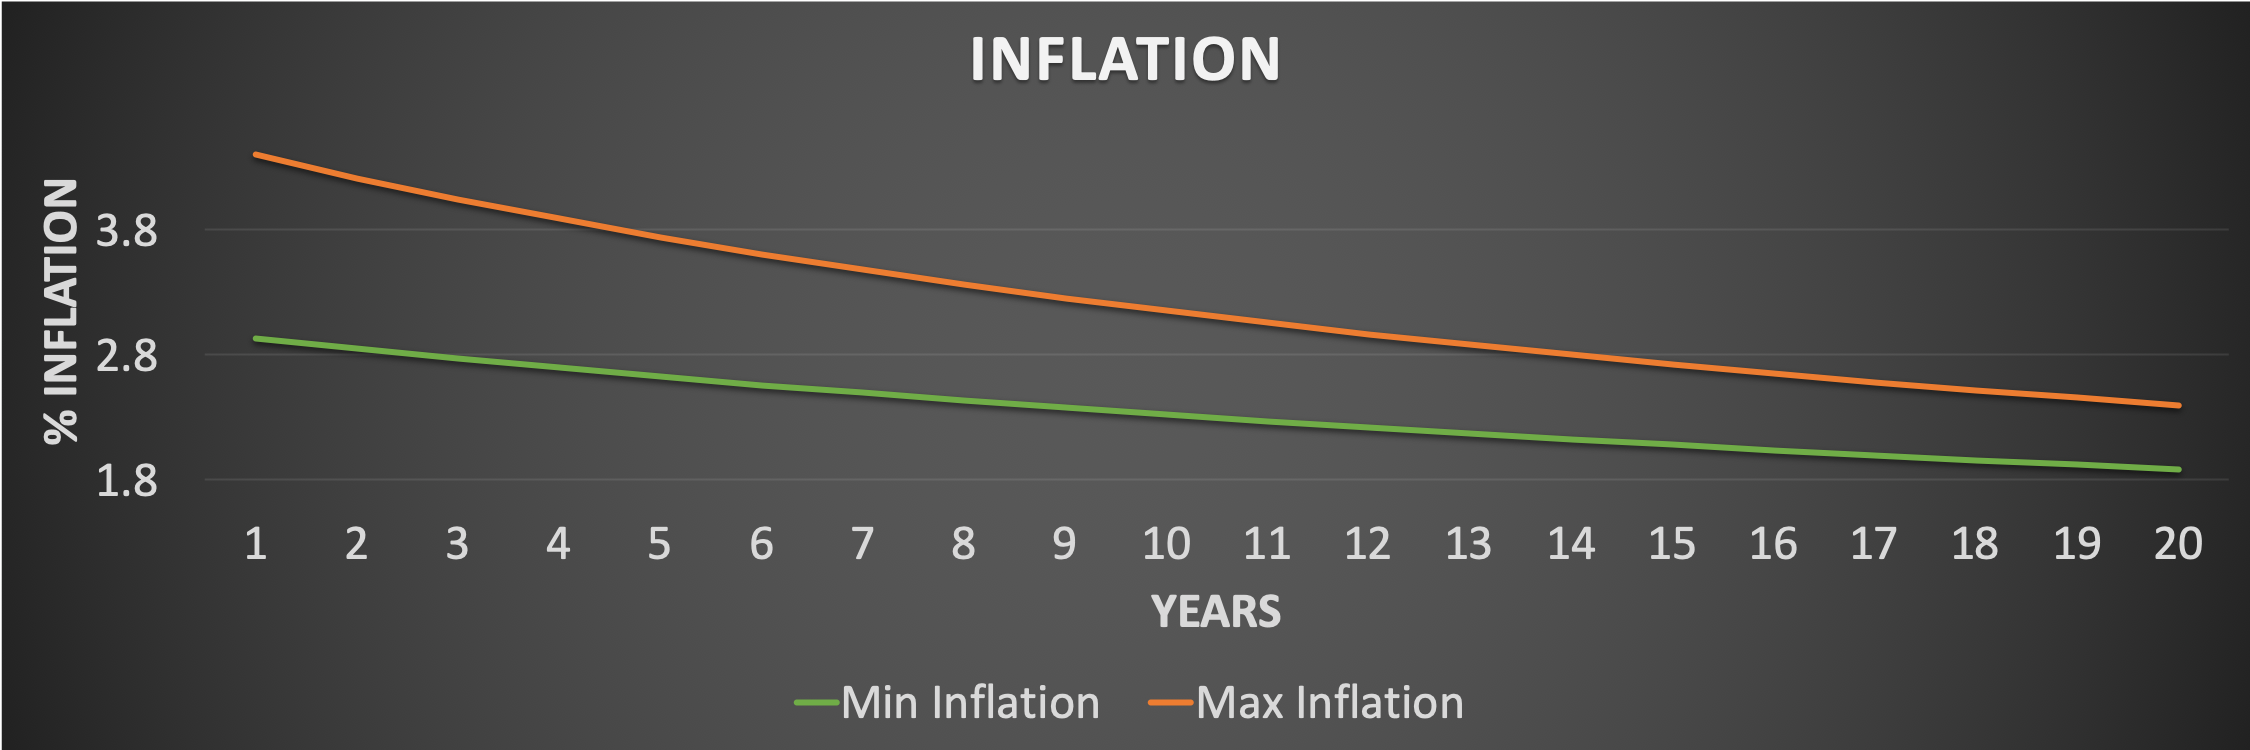
\includegraphics[width=\textwidth]{inflation.png}
	\caption{Min inflation rate after 20 years = 1.88\%, Max inflation 
	rate after 20 years = 2.40\% }
\end{figure}
\noindent
There are different strategies employed by different cryptocurrencies around 
Inflation\footnote{\textit{Spectrecoin differs from Bitcoin and some other 
cryptocurrencies in that we have a constant coin generation scheme 
but a relative inflation that tends to zero over time. There will 
always be an incentive to stake Spectrecoin and the system will never 
rely on fees alone to provide this incentive. It is beyond the scope 
of this paper to have an in-depth discussion about inflation and money 
supply and the nature of money and currencies. Spectrecoin can be seen 
as a ‘medium of exchange’ and the aim is that Spectrecoin will be used 
to buy/sell goods and other fiat currency in its intended use in future 
online cash transfers. Economists discuss and debate this point but some 
level of inflation and value creation appears to be beneficial for long 
term adoption and will prevent Spectrecoin from the potential dangers of 
entering a ‘deflationary spiral’ relaying on fees alone to sustain the 
Spectrecoin ecosystem.}}. There doesn’t seem to be a consensus amongst 
scholars of what might be ‘\textit{the best}’ strategy.
\newpage

\subsection{Total supply (‘outstanding’ amount) over 20 years}
\begin{figure}[ht]
	\centering
	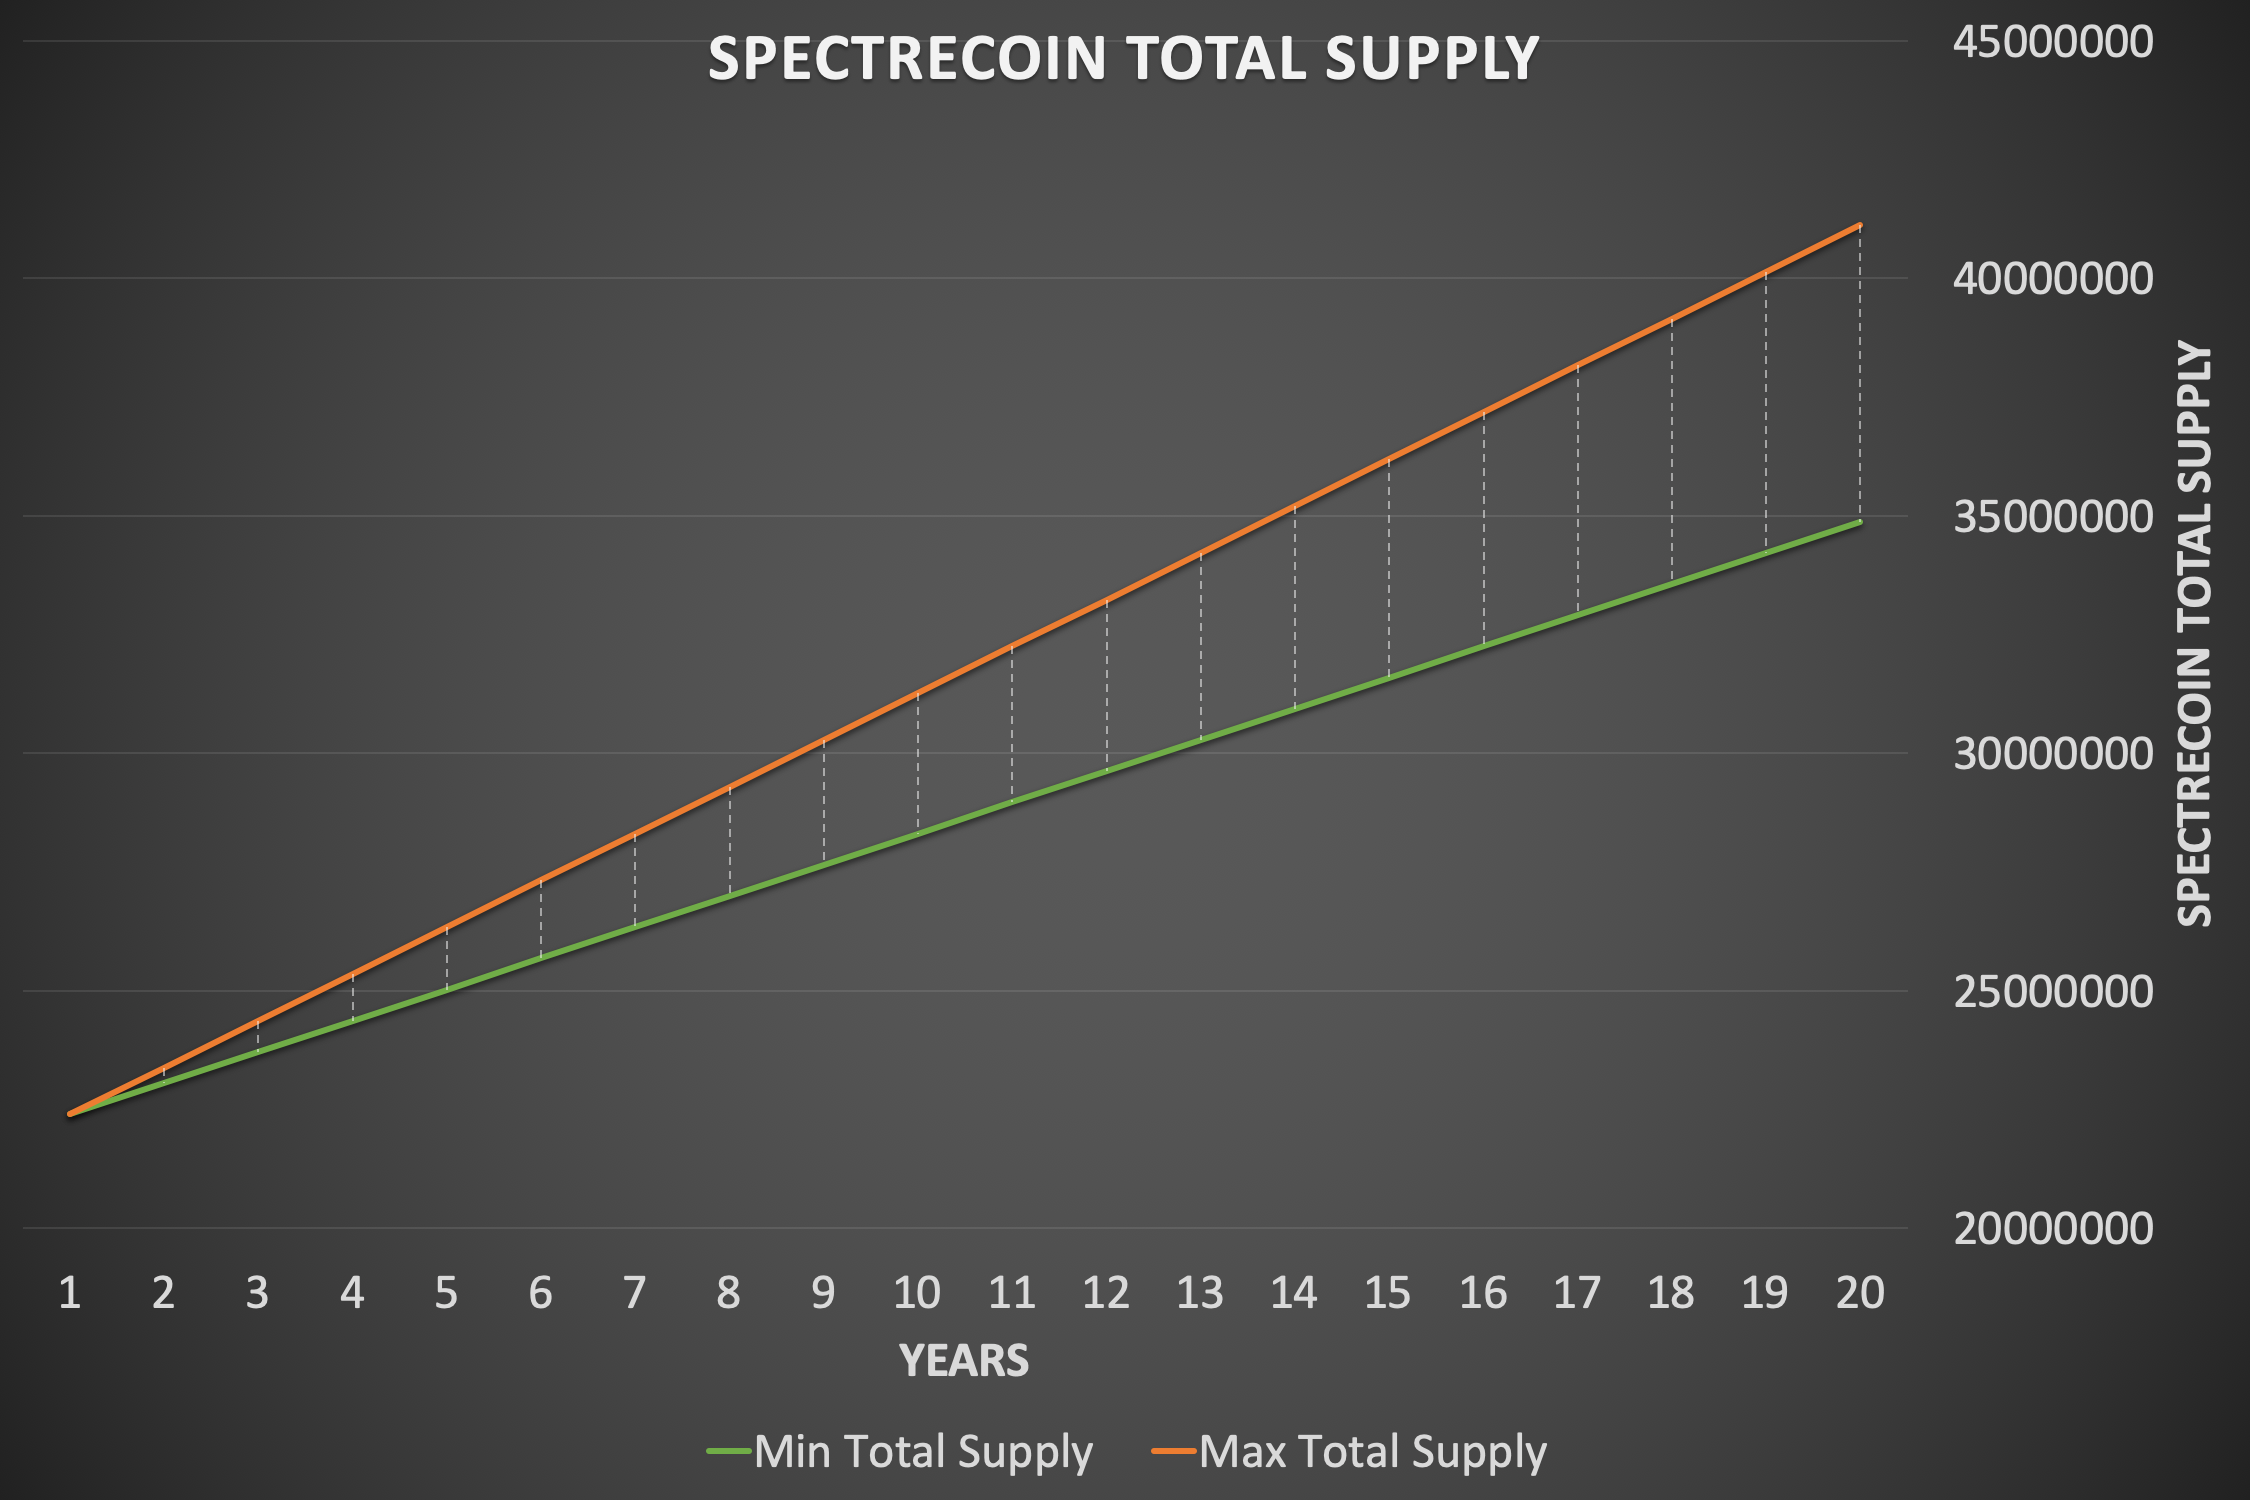
\includegraphics[width=\textwidth]{supply.png}
	\caption{Min supply after 20 years = 34,883,000 XSPEC+SPECTRE - Max 
		supply after 20 years = 41,124,500 XSPEC+SPECTRE}
\end{figure}
\noindent
The block explorer\footnote{https://chainz.cryptoid.info/xspec/} allows you 
to explore the Spectrecoin blockchain and you can see the total supply at any given time.

\subsection{Maturity}
The maturity calculations have changed such that the minimum maturity for
staking and for spending stakes has been increased from 288 to 450 blocks. That means that the new maturity time is approximately $96 seconds * 450 = 12 hours$ and hence the 8-hour maturity rule for staking has been removed. Also, note that the updated maturity rule is also considered for all ATXOs used in the ring signature
of the staked VIN.

\subsection{Reward and Fee Handling}
The stake reward for a PoAS block is 3 SPECTRE and 2 XSPEC for a PoSv3 block.
The fees are the same for both XSPEC and SPECTRE transactions.
\newpage

\subsection{Proof-of-Stake vs. Proof-of-Work}
Spectrecoin uses both PoSv3 and PoAS algorithms to keep the network consensus and to secure and confirm transactions. Both PoSv3 and PoAS appear to be more resilient against various attacks that could be instigated against a Proof-of-Work (PoW) system like Bitcoin, Litecoin and DASH for example. It is also known that PoW systems are susceptible to so called 51\% attacks where a sufficiently funded and motivated attacker can “\textit{take control}” over the network and generate double spend transactions\footnote{https://www.crypto51.app/}. It is more difficult to attack a PoS system in this way as it would be unfeasible to acquire the majority of Spectrecoin in circulation and doing so would undermine the value and remove the incentive for the attack in the first place. There are obviously other attack vectors, such as the recently discovered so called “\textit{Fake Stake}” attack against PoSv3\footnote{https://medium.com/@dsl\_uiuc/fake-stake-attacks-on-chain-based-proof-of-stake-cryptocurrenciesb8b05723f806}. This has since been fixed by the Spectrecoin developers and Spectrecoin is no longer susceptible to such an attack.
\\
\\
\noindent
It is also well known that large PoW driven networks expend huge amounts of energy and appears to lead to some level of centralisation of mining power due to the huge expense involved in mining new blocks. In a recent research paper entitled “\textit{The Bitcoin Mining Network - Trends, Composition, Average Creation Cost, Electricity Consumption \& Sources}” by Christopher Bendiksen \& Samuel Gibbons of CoinShares  Research\footnote{https://coinshares.co.uk/\#mailmunch-pop-792759}, 
it was found that the Bitcoin network expends more energy than the whole country of New Zealand.
\\
\\
\noindent
The report calculated that the global Bitcoin mining industry draws 4.7GW of power every second. Hashing computations for the Proof-of-Work algorithm consumed 4.3GW, up 0.4GW from the last CoinShares report in November 2018. Based on these figures, researchers calculated \textbf{an annual consumption of 41TWh of electricity}. That’s roughly 2.2TWh more than New Zealand – a country of 4.7M people – consumed in 2017, according to the country’s Electricity Authority\footnote{https://www.ea.govt.nz/}.
\\
\\
\noindent
In comparison, Spectrecoin will run on a standard Raspberry Pi and in addition to all the privacy features, Spectrecoin is also truly eco-friendly, sustainable and ‘\textit{green technology}’. The estimated loose upper bound, \textbf{annual 
consumption for a Raspberry Pi running Spectrecoin is 16.6kWh}.

\vspace{5mm} %5mm vertical space

Bitcoin network:\\
$41 TWh = 41*1012 Wh = 41,000,000,000,000 Wh$

\vspace{5mm} %5mm vertical space

Spectrecoin node:\\
$16.6 KWh = 16.6 * 103 Wh = 16,600 Wh * 1000 (nodes) = 16,600,000 Wh$

\vspace{5mm} %5mm vertical space

That means that the whole \textit{Bitcoin network consumes almost \textbf{2.5 million times
more energy} than what an imaginary Spectrecoin network would consume}, assuming
1000 Spectrecoin Raspberry Pi nodes.
\newpage
\noindent
In summary, the PoSv3 / PoAS protocols are both potentially more secure,
immensely more energy efficient and provides for better decentralisation.
It is beyond the scope of this paper to discuss this further and there are
various discussions around the internet if you are interested in the PoW vs.
PoS debate.
\\
\\
\noindent
In the next sections we will explore the different aspects of Spectrecoin in
more detail. We start on the next page with a detailed introduction to the
Spectrecoin privacy features before we go on to discuss Proof-of-Stake v3
(PoSv3) in detail. We move on to explain the privacy features and the new
Proof-of-Anonymous-Stake (PoAS) protocol.